\documentclass[tikz]{standalone}
\usepackage{cancel}
\usepackage{fontspec}
\setmonofont[Scale=MatchLowercase]{DejaVu Sans Mono}
\usetikzlibrary{arrows.meta}

\begin{document}
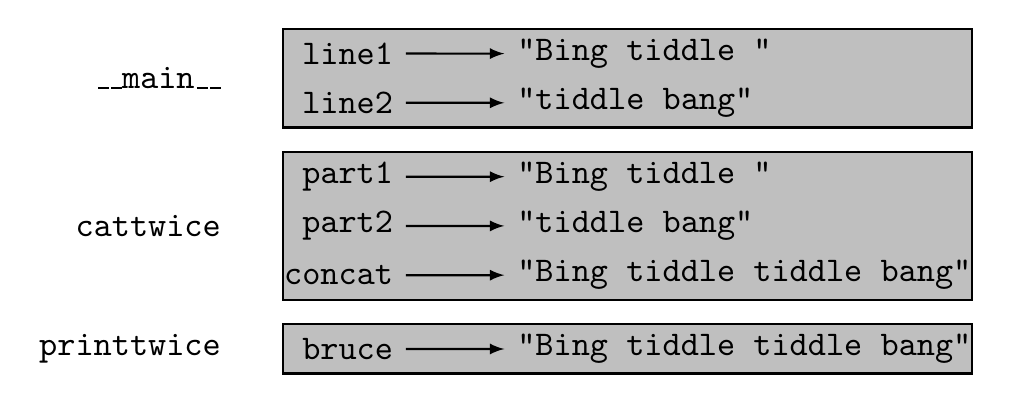
\begin{tikzpicture}[thick, scale=1.25, transform shape]
$\node[anchor=east] at(-4,0){\tt \_\_main\_\_};
\node[draw, fill=lightgray, minimum width=7cm, minimum height=1cm]{};
\node[anchor=east] (l1) at(-2.25, 0.25) {\tt line1};
\node[anchor=west] (l1v) at (-1.25, 0.25) {\tt "Bing tiddle "};
\draw[-latex] (l1) -- (l1v);
\node[anchor=east] (l2) at(-2.25, -0.25) {\tt line2};
\node[anchor=west] (l2v) at (-1.25, -0.25) {\tt "tiddle bang"};
\draw[-latex] (l2) -- (l2v);
\node[anchor=east] at(-4,-1.5){\tt cattwice};
\node[draw, fill=lightgray, minimum width=7cm, minimum height=1.5cm] at(0,-1.5){};
\node[anchor=east] (p1) at(-2.25, -1) {\tt part1};
\node[anchor=west] (p1v) at (-1.25, -1) {\tt "Bing tiddle "};
\draw[-latex] (p1) -- (p1v);
\node[anchor=east] (p2) at(-2.25, -1.5) {\tt part2};
\node[anchor=west] (p2v) at (-1.25, -1.5) {\tt "tiddle bang"};
\draw[-latex] (p2) -- (p2v);
\node[anchor=east] (cc) at(-2.25, -2) {\tt concat};
\node[anchor=west] (ccv) at (-1.25, -2) {\tt "Bing tiddle tiddle bang"};
\draw[-latex] (cc) -- (ccv);
\node[anchor=east] at(-4,-2.75){\tt printtwice};
\node[draw, fill=lightgray, minimum width=7cm, minimum height=0.5cm] at(0,-2.75){};
\node[anchor=east] (b) at(-2.25, -2.75) {\tt bruce};
\node[anchor=west] (bv) at (-1.25, -2.75) {\tt "Bing tiddle tiddle bang"};
\draw[-latex] (b) -- (bv);
$
\end{tikzpicture}
\end{document}
